\section{Projeto de Software}

A partir dos Requisitos Técnicos levantados, foi realizado o projeto de software. O projeto se iniciou com a definição de casos de uso a serem implementados, de forma a satisfazer os requisitos técnicos, em conjunto o diagrama de casos de uso definido pela UML foi elaborado para prover apresentação visual. Em seguida, as informações que devem ser armazenadas pelo sistema foram levantadas e a relação entre elas foi estabelecida, sendo representada no diagrama de entidade-relacionamento. O passo seguinte foi a definição da arquitetura de software do sistema.

No projeto a arquitetura de microsserviços foi escolhida como padrão para o sistema. Essa arquitetura define padrões de modularização do sistema em componentes pequenos e altamente especializados, conferindo facilidades de manutenção e escalabilidade em contraste com a arquitetura de monólito. Em contrapartida, o sistema é mais complexo de se implementar e implantar, devido a separação dos módulos, contudo, considerando o desejo de continuar este projeto após a entrega e os padrões de mercado atuais a abordagem de microsserviços é considerada a mais adequada. 

Definida a arquitetura, cada módulo do sistema foi especificado e foi elaborado o diagrama de componentes, definido pela UML, para ilustrar os pontos de comunicação e componentização da solução completa. Nessa etapa foram definidas as tecnologias a serem empregadas em cada módulo, a justificativa das escolhas é apresentada após o detalhamento dos componentes da arquitetura de software. O projeto de implantação foi então realizado, com planejamento da disponibilização do sistema de software com ferramentas de computação de nuvem disponíveis no mercado.

% TODO: Adicionalmente, foram desenhados protótipos das interfaces que o usuário tem contato, e estão disponibilizadas no Apêndice \ref{appendice:prototipos}

\subsection{Especificação dos Casos de Uso}

Na definição dos casos de uso do projeto foram definidos dois atores que interagem com o sistema de software a ser desenvolvido, identificados como 
usuário e dispositivo. O usuário representa o utilizador humano do sistema a ser desenvolvido, responsável por todas as interações humanas necessárias. 

O usuário se comunica com o sistema por duas interfaces, uma aplicação web, que se comunica diretamente com o sistema, e um aplicativo para smartphone, necessário para configurações iniciais do dispositivo. O dispositivo representa o sistema hardware de controle e monitoramento, também desenvolvido neste projeto. Em relação ao sistema de software, ele é tratado como um ator com suas devidas interações; seu projeto e especificações são discutidos na seção destinado ao projeto de hardware.

Segue a especificação dos casos de uso em si, contendo a identificação de cada caso de uso, sua breve descrição, enumeração dos passos que o definem e 
listagem dos requisitos técnicos relacionados ao caso de uso. Com caráter ilustrativo, o Diagrama de Casos de Uso da UML é apresentado na figura \ref{fig:diagrama_caso_de_usos}.

\subsubsection*{UC - 1: Registro de Dispositivo} 

Descrição: ao obter um novo dispositivo, o usuário deve configurar seu acesso à rede Wi-Fi e registrá-lo, de modo que o sistema reconheça que aquele 
dispositivo pertence ao usuário.
\begin{enumerate}
    \item Usuário acessa aplicativo em seu smartphone
    \item Sistema autentica acesso do usuário
    \item Aplicativo se conecta ao dispositivo
    \item Usuário informa configurações da rede Wi-Fi
    \item Aplicativo envia informações da rede para dispositivo
    \item Dispositivo se conecta na rede e se prepara para receber mensagens do sistema
    \item Aplicativo envia informações do dispositivo para o sistema
    \item Sistema cadastra informações do dispositivo e usuário
\end{enumerate}
Requisito relacionado: SW-F-12

\subsubsection*{UC - 2: Cadastro de Receitas}
Descrição: fluxo de cadastro de receitas.
\begin{enumerate}
    \item Usuário acessa tela de listagem de receitas
    \item Sistema exibe todas as receitas referentes ao usuário
    \item Usuário seleciona opção “Criar Receita” e acessa tela de cadastro de receita
    \item Usuário informa nome, estilo e observações da receita e clica em “Salvar”
    \item Sistema cadastra a receita no banco de dados
\end{enumerate}
Requisito relacionado: SW-F-4

\subsubsection*{UC - 3: Cadastro de Lotes}
Descrição: fluxo de cadastro de lotes, perfis de controle e associação de lote a um dispositivo.
\begin{enumerate}
    \item Usuário acessa tela de listagens de receitas
    \item Sistema exibe todas as receitas referentes ao usuário
    \item Usuário escolhe uma receita e seleciona a opção “Criar Lote”, e acessa a tela de cadastro de lote
    \item Sistema carrega listagem de perfis de controle já cadastrados e dispositivos do usuário
    \item Usuário informa identificação e observações do lote
    \item Usuário escolhe um perfil de controle já existente ou cria um novo perfil, informando uma identificação e cada um dos passos de controle (instante e valor alvo de temperatura)
    \item Usuário seleciona qual dispositivo irá controlar a produção do lote
    \item Usuário clica em “Salvar”
    \item Sistema cadastra lote, perfil de controle (caso novo), associação de lote e perfil de controle, e associação de lote e dispositivo
    \item Sistema envia informações do lote para dispositivo selecionado
\end{enumerate}
Requisitos relacionados: SW-F-5 e SW-F-6.

\subsubsection*{UC - 4: Envio das informações do Lote para Dispositivo}
Descrição: fluxo de envio das informações do lote para o dispositivo associado ao controle daquele lote.
\begin{enumerate}
    \item Dispositivo recebe informações do lote que foi associado por tópico de mensagens
    \item Dispositivo salva informações localmente
    \item Quando pronto, dispositivo inicia rotina de monitoramento e controle
\end{enumerate}    
Requisito relacionado: HW-F-5

\subsubsection*{UC - 5: Envio das informações do Dispositivo para o Sistema}
Descrição: fluxo de envio das informações obtidas pelo monitoramento do processo pelo dispositivo para o sistema.
\begin{enumerate}
    \item Dispositivo envia dados coletados para o sistema
    \item Sistema processa dados e salva informações no banco de dados
\end{enumerate}    
Requisitos relacionados: HW-F-6, SW-F-9

\subsubsection*{UC - 6: Visualização das Informações dos Lotes}
Descrição: fluxo para visualização das informações gerais e de evolução dos lotes correntes e passados
\begin{enumerate}
    \item Usuário acessa tela de listagem dos lotes
    \item Sistema exibe todas os lotes referentes ao usuário
    \item Usuário escolhe um lote e seleciona a opção “Ver Informações”, acessando a tela de informações do lote
    \item Sistema exibe informações gerais sobre o lote, como identificação, receita, observações, status, data de início, data de término, densidades relativas inicial e final/atual, estimativa de teor alcoólico, pH final/atual, temperatura final/atual.
    \item Sistema exibe um gráfico com as variáveis monitoradas em relação ao tempo
    \item Caso usuário clique em “Baixar Dados”, sistema efetua o download dos dados do gráfico em arquivo de texto
\end{enumerate}    
Requisitos relacionados: SW-F-2, SW-F-3, SW-F-8, SW-F-11

\begin{figure}[ht]
    \centering
    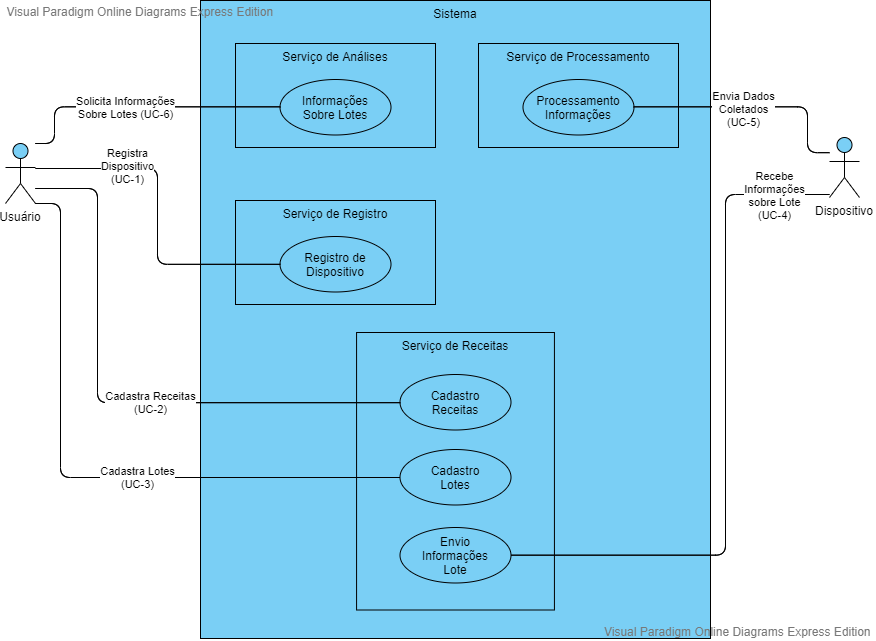
\includegraphics[scale=0.45]{figuras/projeto/software/diagrama_casos_de_uso.png}
    \caption{Diagrama de Casos de Uso.}
    \label{fig:diagrama_caso_de_usos}
\end{figure}

\subsection{Modelo de Entidade-Relacionamento}

O Modelo Entidade Relacionamento descreve como as informações são organizada no sistema e como o banco de dados do sistema é estruturado. 
Cada entidade no modelo representa um tipo de informação que é produzida e consumida pelo sistema, na execução dos casos de uso. 

Todas as informações são armazenadas em um banco de dados relacional, dividido em schemas que atuam como partições de dados em diferentes domínios. 
Foram definidos três domínios, traduzidos em schemas no banco de dados, para os dados: user, recipe e control. O schema user contém as informações 
referentes aos usuários e dispositivos do sistema; o domínio recipe contempla as entidades relacionadas às receitas e lotes de produção, assim como 
os dados coletados em cada execução de uma receita; e o schema control, por fim, os perfis de controle que são seguidos pelo dispositivo durante 
seu funcionamento. A separação das entidades em domínios é importante na arquitetura de microsserviços para assegurar que cada serviço tenha 
controle apenas às informações de sua competência. 

A definição das entidades e seus relacionamentos é ilustrada pelo Diagrama Entidade Relacionamento da figura \ref{fig:diagrama_entidade_relacionamento}, com destaque em cor para cada um dos schemas determinados.

\subsection{Arquitetura de Software}

A arquitetura de software do projeto foi estruturada tendo como base o fluxo da informação como especificado nos casos de uso e os conceitos de arquitetura de microsserviços. Dessa forma, foram definidas quatro camadas para organizar os sistemas a serem implementados: Camada de Interface, contemplando as interfaces utilizadas diretamente pelos atores; Camada Intermediária, contendo um API Gateway para isolar os microsserviços das interfaces e um message broker para intermediar a comunicação entre dispositivo e sistema; Camada de Negócio, contendo os microsserviços que exercem as regras de negócio do sistema; e Camada de Persistência, com os serviços de armazenamento de dados. Os componentes de cada camada são descritos em detalhes quanto a suas responsabilidades e detalhes de implementação em sequência. A arquitetura completa é representada visualmente pelo Diagrama de Componentes da figura \ref{fig:diagrama_componentes}.

\subsubsection{Camada de Interface}
A Camada de Interface (figura \ref{fig:camada_interface}) contém os componentes que fornecem interface direta aos atores definidos na modelagem de casos de uso. Sua função, portanto, reside na interação com os atores e comunicação de suas ações para a próxima camada, a Camada Intermediária. São três componentes de interface que compõe essa camada: Aplicação Front-end, Aplicação Mobile e o Software Embarcado no dispositivo. 

\begin{figure}[h]
    \centering
    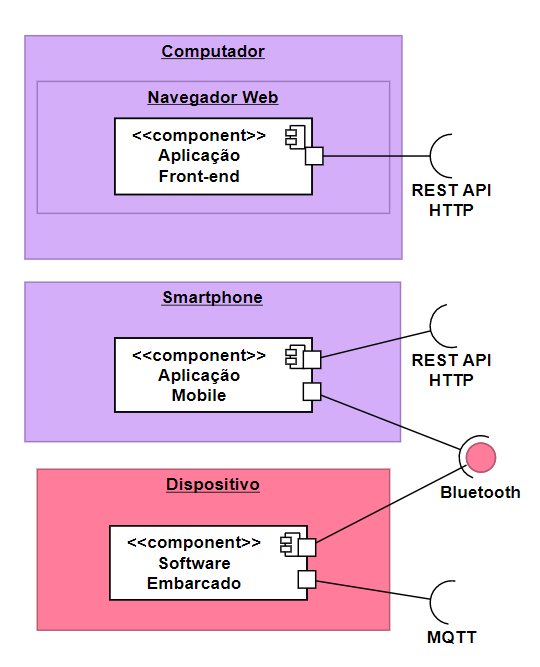
\includegraphics[scale=0.50]{figuras/projeto/software/camada_interface.PNG}
    \caption{Camada de Interface.}
    \label{fig:camada_interface}
\end{figure}

A Aplicação Front-end é executada pelo navegador web do usuário do sistema, e permite que ele realize o cadastro e gerenciamento de todas as informações referentes ao sistema, como receitas, perfis de controle e lotes, ela também permite que o usuário visualize os dados gerados pelo dispositivo em formato de gráficos e tabelas. Essa aplicação contém o componente gráfico das telas que o usuário utilizará e algumas regras de validação simples, como campos obrigatórios de cadastro. As ações do usuário são traduzidas em requisições HTTP que são enviadas para o Serviço de API Gateway, na próxima camada. 

A Aplicação Mobile foi a solução encontrada para intermediar a comunicação entre usuário e dispositivo, suas principais funções são: enviar as informações necessárias para conexão à rede Wi-Fi do usuário, que é realizado pela tecnologia de bluetooth, e informar o sistema que aquele dispositivo foi ativado por determinado usuário. Após essa configuração, o usuário poderá associar um lote de uma receita para o dispositivo monitorar e controlar, e o dispositivo deve estar pronto para se comunicar com o sistema por meio de mensagens.

O Software Embarcado no dispositivo, além das funcionalidades de monitoramento e controle, que são detalhadas nas seções de Modelagem de Controle e Projeto de Hardware, deve ser capaz de se comunicar via tecnologia bluetooth com a Aplicação Mobile, e enviar e receber mensagens via protocolo MQTT com o Message Broker da Camada Intermediária. O dispositivo deve enviar mensagens com os dados que estão sendo coletados durante a fermentação, como temperatura, densidade relativa e pH, e receber informações sobre um novo lote que foi alocado para ele realizar o controle.

\subsubsection{Camada Intermediária}

Toda a comunicação entre os atores e o sistema é realizada por mediação da Camada Intermediária (figura \ref{fig:camada_intermediaria}). O tráfego pode ocorrer pelos protocolos HTTP ou MQTT. O fluxo por HTTP é mediado pelo Serviço de API Gateway, que roteia as requisições externas para os devidos microsserviços, enquanto que o fluxo MQTT, composto por mensagens, é controlado pelo Message Broker, que organiza as mensagens nos fluxos dispositivo para sistema e sistema para dispositivo.

\begin{figure}[h]
    \centering
    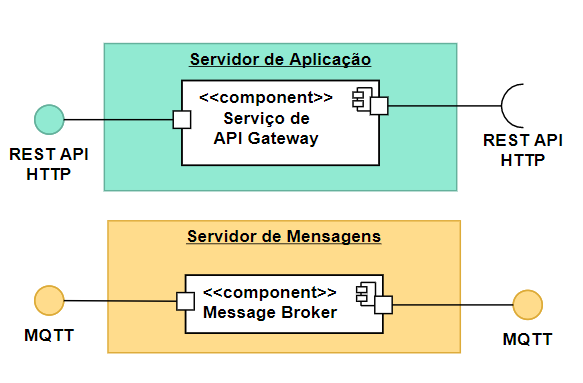
\includegraphics[scale=0.50]{figuras/projeto/software/camada_intermediaria.PNG}
    \caption{Camada Intermediária.}
    \label{fig:camada_intermediaria}
\end{figure}

O Serviço de API Gateway funciona como um serviço de proxy reverso que, além centralizar as solicitações do usuário, consolida o resultado de cada microsserviço necessário para atender uma demanda. Apesar de ser um serviço muito simples, ele é importante por questões de segurança, uma vez que apenas um endereço fica exposto externamente e a autenticação externa é centralizada nele, e também por questões de escala futura, sendo mais fácil implantar um balanceador de carga ou sistema de fila de processamento com essa separação de serviços, caso seja necessário no futuro.

O Message Broker é simplesmente um corretor de mensagens, que opera sobre o protocolo MQTT, e é responsável pelo recebimento, entrega e armazenamento das mensagens que trafegam no sistema. O protocolo MQTT foi escolhido por ser extremamente leve e desenvolvido especialmente para o uso em Internet das Coisas.
    
\subsubsection{Camada de Negócio}

Os microsserviços do sistema, que aplicam as regras de negócios, estão presentes na Camada de Negócio. Os componentes dessa camada são responsáveis pela validação de consistência das informações, interação com o banco de dados na Camada de Persistência através da interface ODBC, e processamento dos dados coletados pelo dispositivo. Cada microsserviço que compõe essa camada é especializado e responsável por uma quantidade restrita de entidades, prezando-se pelo baixo acoplamento do sistema. Simplificando a implantação do sistema, alguns serviços foram agrupados em um mesmo servidor, mediante sua afinidade em relação às informações em que se especializa.

O Servidor de Registro (figura \ref{fig:camada_negocios_registro}) comporta os Serviços de Usuários e de Dispositivos, que são responsáveis pelo cadastro, recuperação, atualização e deleção  (CRUD, em inglês) dos registros de usuários e registros, respectivamente. Além disso, o Serviço de Usuários controla a associação entre um usuário e seus dispositivos.

\begin{figure}[h]
    \centering
    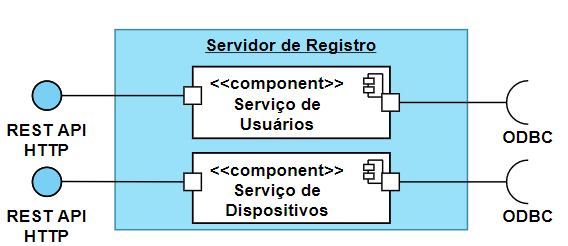
\includegraphics[scale=0.50]{figuras/projeto/software/camada_negocios_registro.PNG}
    \caption{Camada de Negócio - Servidor de Registros.}
    \label{fig:camada_negocios_registro}
\end{figure}

Os Serviços de Controle, Receitas e Lotes também exercem a responsabilidade sobre o CRUD de perfis de controle, receitas e lotes, respectivamente, e foram agrupados no Servidor de Receitas (figura \ref{fig:camada_negocios_receita}). O Serviço de Lotes também realiza a associação de um lote com o dispositivo e envia todas as informações necessárias para o controle do lote da receita para o dispositivo que foi associado, essa comunicação é realizada por meio de mensagens sob o protocolo MQTT, que serão consumidas pelo dispositivo conectado à Internet.

\begin{figure}[h]
    \centering
    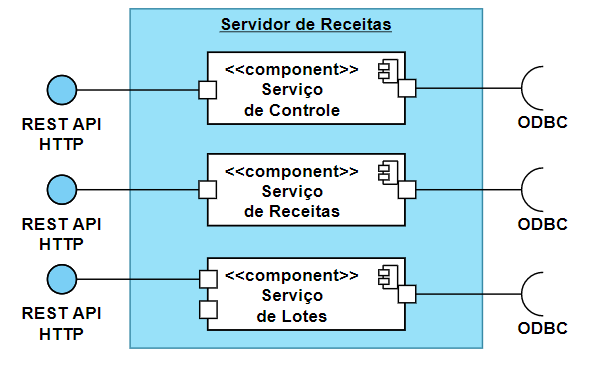
\includegraphics[scale=0.50]{figuras/projeto/software/camada_negocios_receita.PNG}
    \caption{Camada de Negócio - Servidor de Receitas.}
    \label{fig:camada_negocios_receita}
\end{figure}

A figura \ref{fig:camada_negocios} ilustra os demais serviços da Camada de Negócios. O Serviço de Análises empenha função analítica sobre os dados coletados que foram consolidados, fornecendo relatórios de desempenho para o usuário, além de dados para serem exibidos na Aplicação Web. O Serviço de Processamento, ou Processador, acessa os dados enviados pelo dispositivos ao Message Broker e aplica as transformações necessários para consolidar as informações no banco de dados. Adicionalmente, um Serviço de Autenticação foi incluído para atender às necessidades de segurança dos dados e controle de acesso ao sistema.
    
\begin{figure}[h]
    \centering
    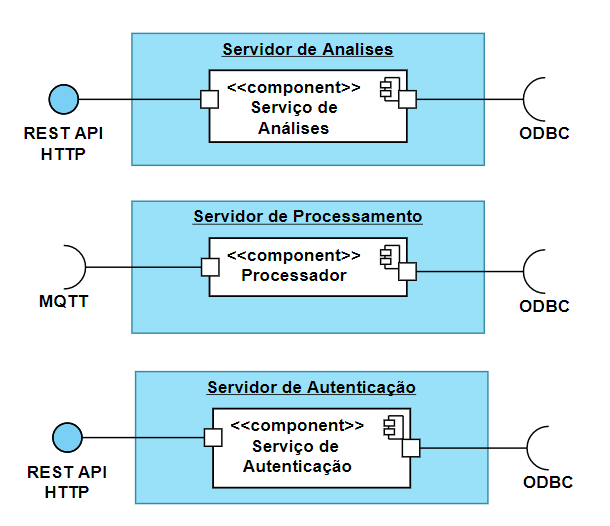
\includegraphics[scale=0.50]{figuras/projeto/software/camada_negocios.PNG}
    \caption{Camada de Negócio - Servidores de Análises, Processamento e Autenticação.}
    \label{fig:camada_negocios}
\end{figure}

\subsubsection{Camada de Persistência}

A Camada de Persistência (figura \ref{fig:camada_persistencia}) abriga os serviços de armazenamento de dados necessários ao sistema. Neste projeto, está previsto apenas um servidor de banco de dados relacional, discutido em maior detalhe na Modelagem de Entidade-Relacionamento.

\begin{figure}[h]
    \centering
    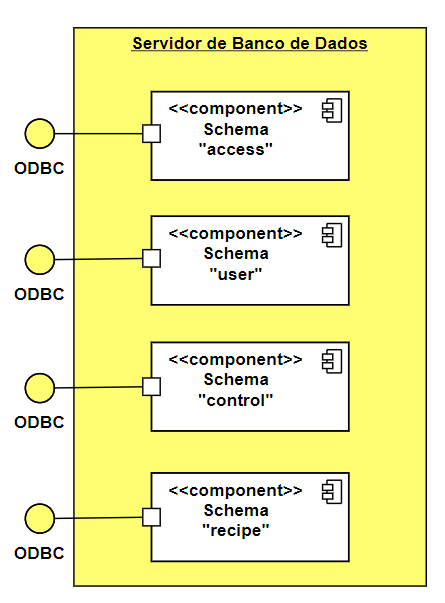
\includegraphics[scale=0.50]{figuras/projeto/software/camada_persistencia.PNG}
    \caption{Camada de Persistência.}
    \label{fig:camada_persistencia}
\end{figure}

\begin{figure}[ht]
    \centering
    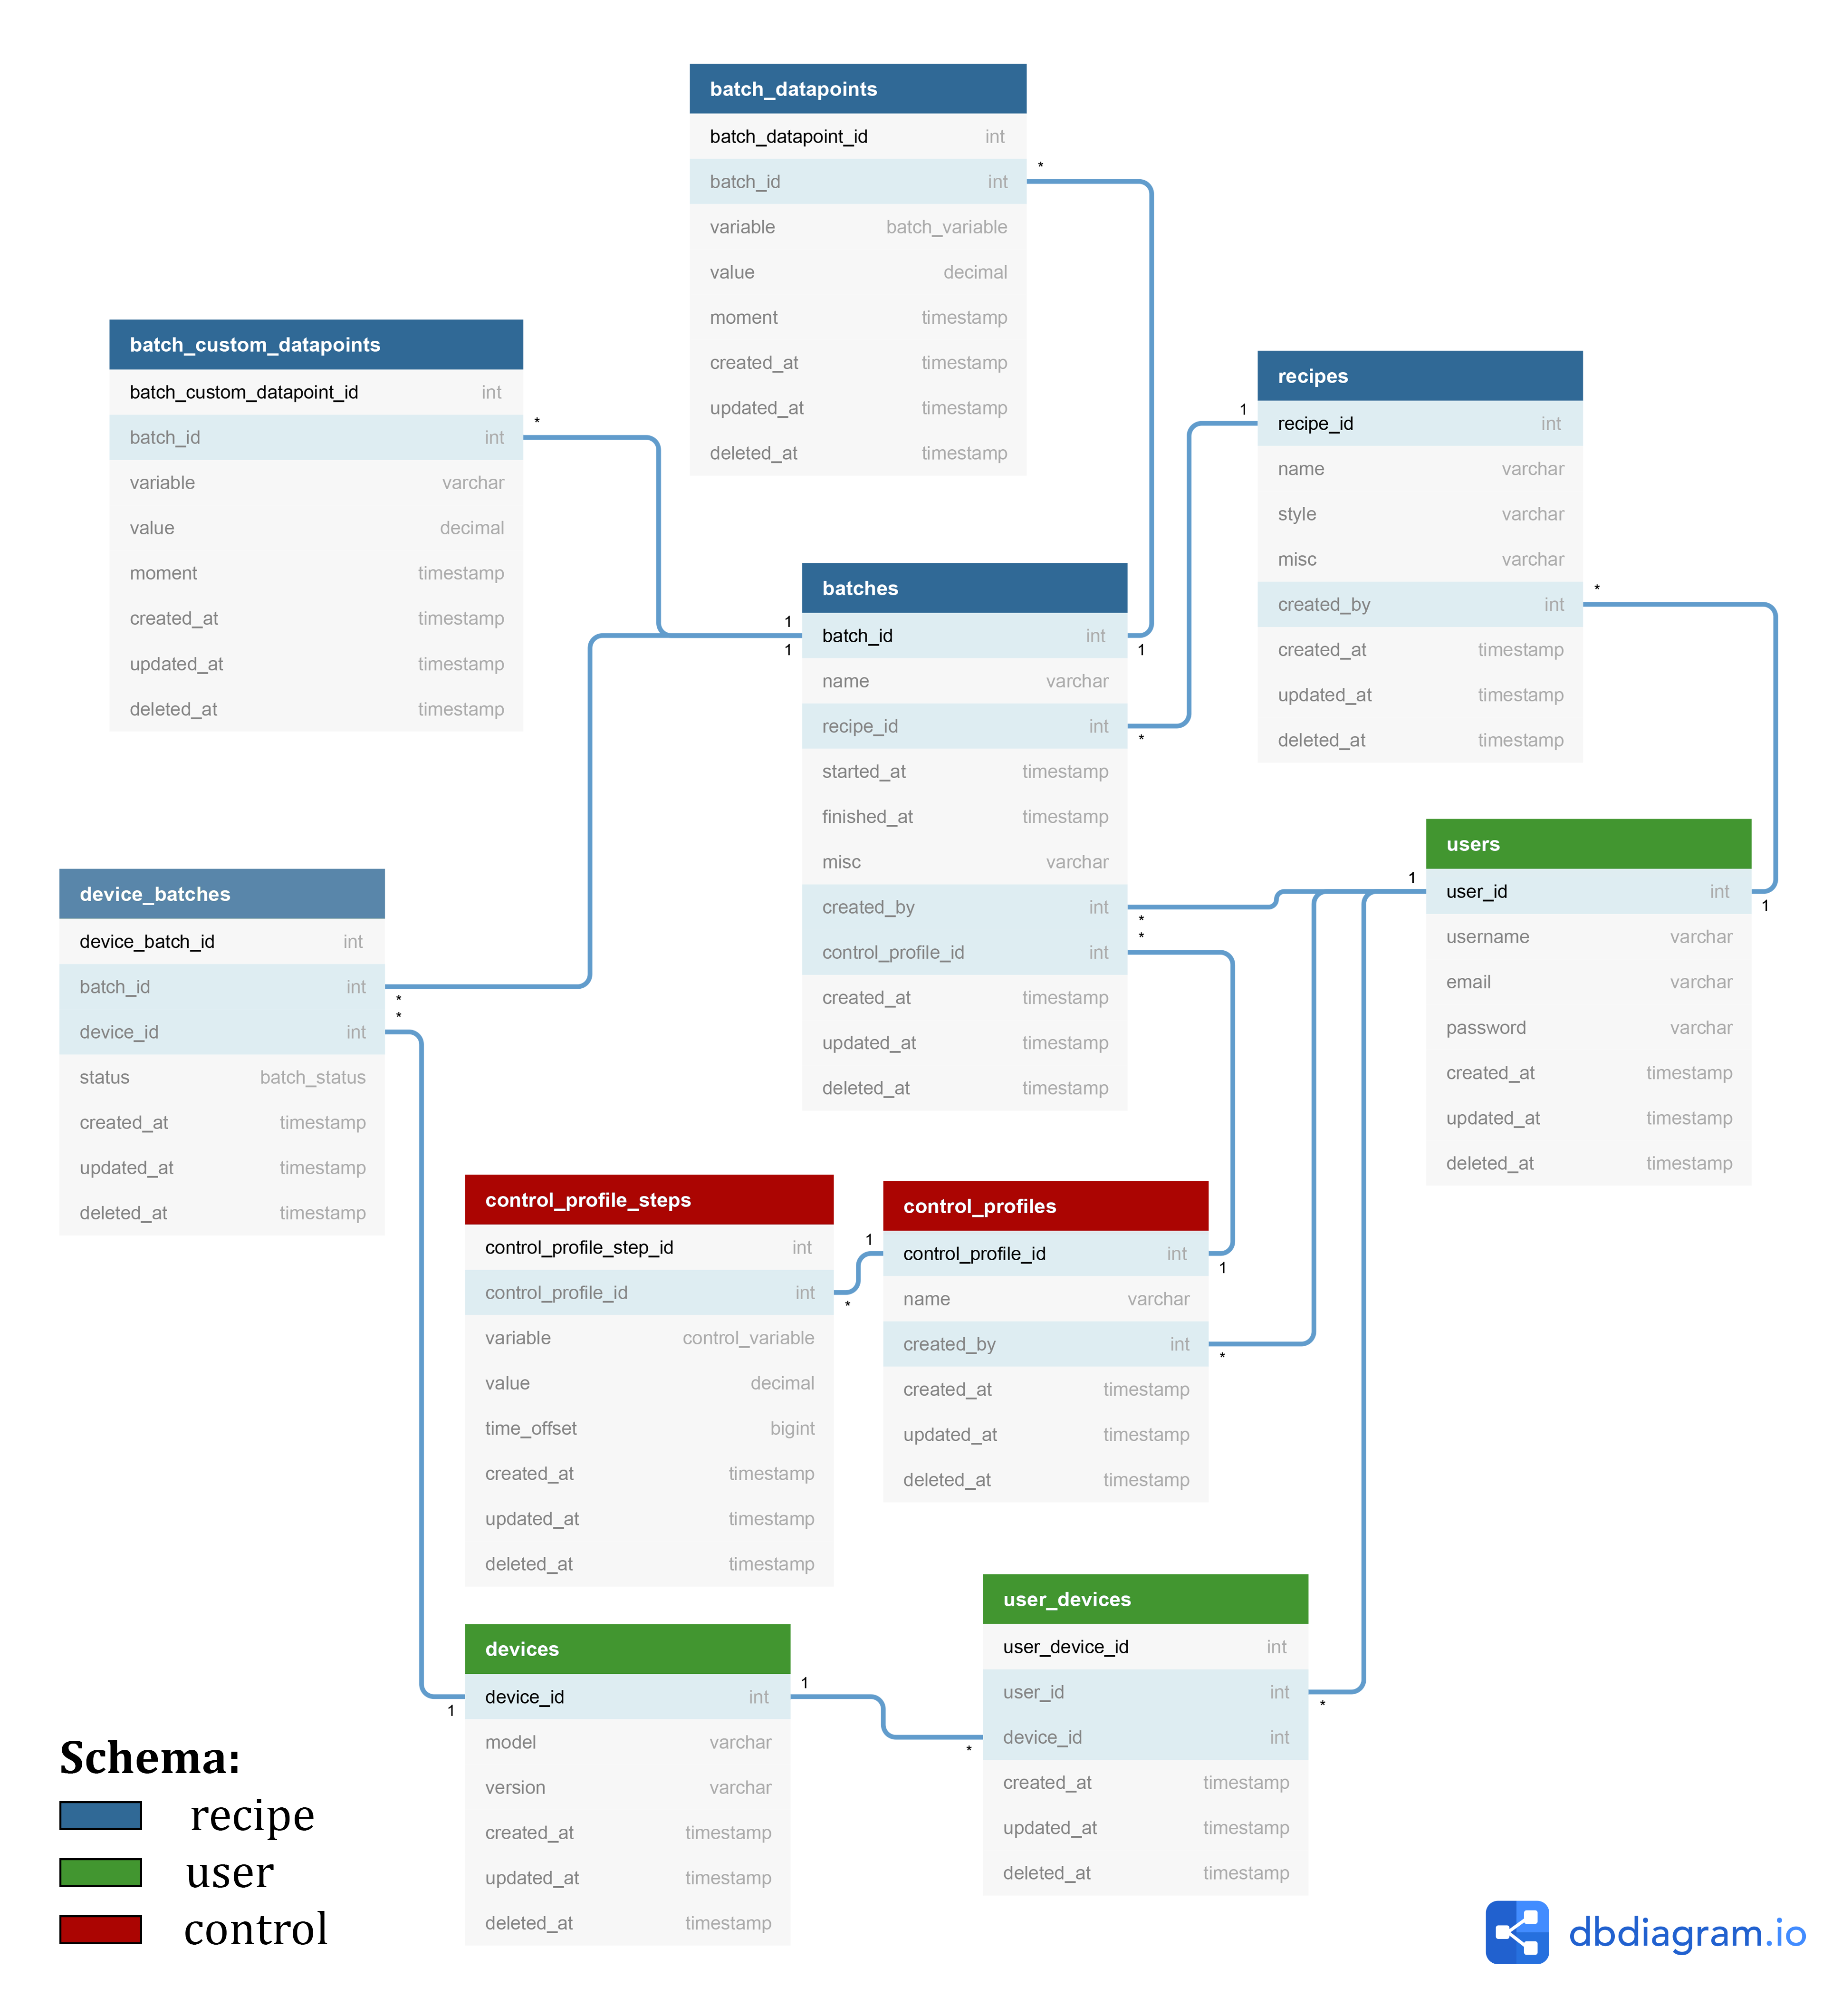
\includegraphics[scale=0.15]{figuras/projeto/software/banco_de_dados.png}
    \caption{Diagrama de Entidade-Relacionamento.}
    \label{fig:diagrama_entidade_relacionamento}
\end{figure}

\begin{figure}[ht]
    \centering
    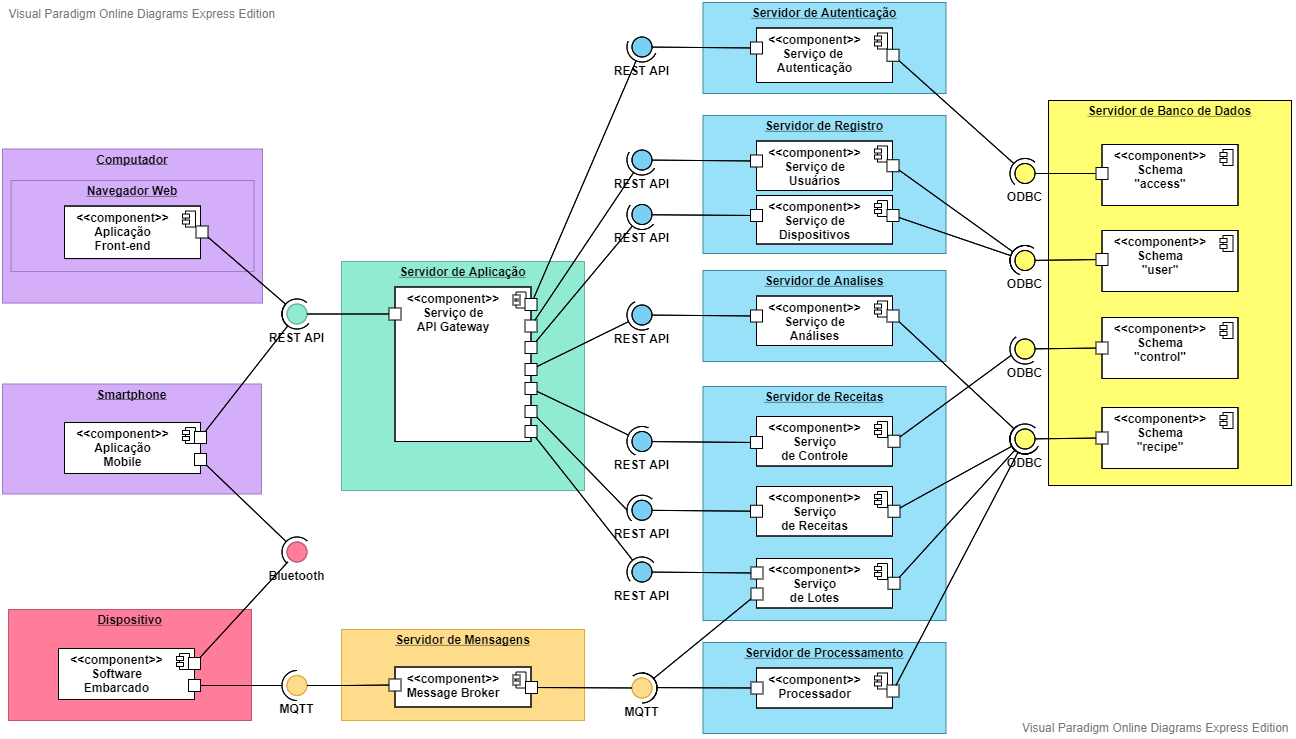
\includegraphics[scale=0.50, angle=270]{figuras/projeto/software/diagrama_componentes.png}
    \caption{Diagrama de Componentes.}
    \label{fig:diagrama_componentes}
\end{figure}

\subsection{Definição de Tecnologias}

As tecnologias a serem utilizadas na implementação implantação deste projeto foram definidas levando em consideração sua adequação e familiaridade dos autores. Dessa forma, foi determinada a utilização da linguagem de programação Python para implementar os microsserviços e as lógicas necessárias no API Gateway. Utilizando o Python, é possível prover de forma simples e com poucos recursos uma API REST utilizando o framework Flask executado com o servidor Gunicorn. A segurança da aplicação segue padrão OAuth 2.0 implementado pela biblioteca oauthlib.

Definiu-se a utilização da biblioteca React da linguagem JavaScript para desenvolvimento da interface da Aplicação Web, utilizando também a biblioteca chart.js para construção de gráficos. Para a interface do Aplicativo Mobile foi definida a linguagem Java, para utilização em smartphones Android. O banco de dados relacional escolhido foi o PostgreSQL. 

% TODO: Melhorar...

\subsection{Projeto de Implantação}

